\chapterimage{chapter_head_1.pdf} 
\chapter{Programación de un juego sin gráficos}

En este capítulo, se darán las instrucciones para la realización paso a paso un videojuego sin usar el sistema gráfico de la NDS.

La lista de ejercicios y el tiempo estimado (en minutos) para su realización se muestran en la Tabla \ref{c4_tab:ejercios}.

\begin{table}[t]
\centering
\caption{Ejercicios del capítulo y tiempo estimado para su realización.}
\begin{tabular}{|c|c|}
\hline 
Ejercicio & Tiempo \\ 
\hline 
 4.1 & 10' \\ 
 4.2 & 20' \\ 
 4.3 & 30' \\ 
 4.4 & 20' \\ 
 4.5 & 10' \\ 
 4.6 & 10' \\ 
 4.7 & 10' \\ 
 4.8 & 10' \\ 
\hline 
\end{tabular} 
\label{c4_tab:ejercios}
\end{table}

% ---------------------------------------------------------
% ---------------------------------------------------------
\section{Descripción del juego}
El juego que se va a realizar es una versión simplificada del típico juego de carreras de caballos que se solían encontrar en las ferias itinerantes. La Figura \ref{fig_c4_caballos}\footnote{La imagen se ha obtenido en la siguiente web: \url{http://www.parquedebolas.com/images/productos/gran/523000002.jpg}} muestra un ejemplo de este tipo de juego. En este juego, el usuario debe introducir bolas en unos agujeros, y según el agujero donde ha caído la bola, el caballo irá más o menos deprisa. Gana el caballo que antes llegue a la meta.

\begin{figure}[t]
	\centering
	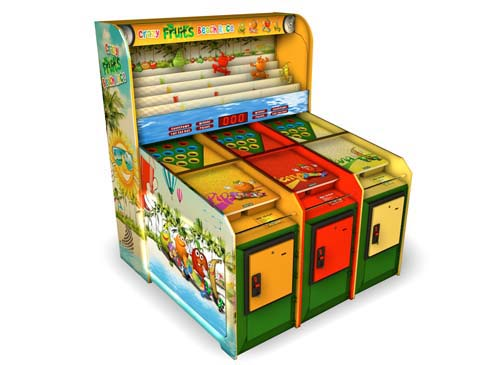
\includegraphics[height=7cm]{Figuras/C4/c4_caballos.jpg}
	\caption{Juego de las carreras de caballos.}
	\label{fig_c4_caballos}
\end{figure}

En la versión que se va a desarrollar se usarán los conceptos aprendidos en el capítulo 3. En la pantalla superior se mostrará la carrera. La pantalla se dividirá en 4 carriles horizontales, uno por caballo. Para representar cada caballo se usará una letra. Al inicio los 4 caballos se situarán en la primera columna de la pantalla (columna 0). Ganará el primer caballo que alcance la meta situada en la última columna de la pantalla (columna 31).

En la pantalla inferior habrá un mensaje indicando el dinero que tiene el jugador. Al inicio el jugador tendrá 1000 euros.

También existirán cuatro botones, uno por caballo. El jugador deberá pulsar en uno de los cuatro botones para apostar por un caballo determinado. La apuesta es de 100 euros. Si el caballo por el que ha apostado el jugador gana, se obtendrán 200 euros que serán añadidos al dinero total. Si gana otro caballo, el jugador perderá ese dinero.

El juego continuará hasta que el jugador se quede sin dinero o alcance la cifra de 10 000 euros.

\section{Desarrollo del juego}

\begin{example}
El siguiente listado (\textit{caballos\_inicial.c}) muestra el esqueleto del programa que puedes usar para empezar:
\begin{lstlisting}
#include <nds.h>
#include <stdio.h>

void MostrarCaballos(int posicion_caballos[]);
void MostrarBotones();
void MostrarDinero(int dinero);

int main(void)
{
  PrintConsole pantalla_sup, pantalla_inf;
  videoSetMode   (MODE_0_2D);
  videoSetModeSub(MODE_0_2D);
  consoleInit (&pantalla_sup, 3, BgType_Text4bpp, 
               BgSize_T_256x256, 31, 0, true, true);
  consoleInit (&pantalla_inf, 3, BgType_Text4bpp, 
               BgSize_T_256x256, 31, 0, false, true);

  int posicion_caballos[4];
  for (int i=0; i<4; i++)
    posicion_caballos[i] = 0;
    
  int dinero = 1000;   

  while(1)
  {
    consoleSelect  (&pantalla_sup);
    MostrarCaballos(posicion_caballos);
    consoleSelect  (&pantalla_inf);
    MostrarDinero  (dinero);
    MostrarBotones ();
  }
}

void MostrarCaballos(int posicion_caballos[])
{
  iprintf("\x1b[2;%dHA", posicion_caballos[0]);
  iprintf("\x1b[8;%dHB", posicion_caballos[1]);
  iprintf("\x1b[14;%dHC",posicion_caballos[2]);
  iprintf("\x1b[20;%dHD",posicion_caballos[3]);
}

void MostrarBotones()
{
  iprintf("\x1b[10;1HApuesta por un caballo: ");
  iprintf("\x1b[12;4H----- ----- ----- -----");
  iprintf("\x1b[13;4H- A - - B - - C - - D -");
  iprintf("\x1b[14;4H----- ----- ----- -----");
}

void MostrarDinero(int dinero)
{
  iprintf("\x1b[2;1HTienes %d euros", dinero);
}
\end{lstlisting}
\end{example}
	
Como se puede comprobar por el código anterior, los cuatro carriles para mostrar la evolución de los caballos estarán en las filas, 2, 8, 14 y 20 de la pantalla superior. En la fila 2 de la pantalla inferior se mostrará un mensaje indicando el dinero que tiene el jugador. En las filas 12, 13 y 14 se mostrarán los botones para apostar por los caballos.

\begin{exercise}
	Crea un nuevo proyecto usando el código \textit{caballos\_inicial.c} y comprueba que funciona correctamente.
\end{exercise}

Para crear el programa completo debes resolver los siguientes ejercicios en el orden establecido. En primer lugar debes crear el código necesario para que los caballos se muevan hacia la meta. Al inicio todos los caballos tendrán una velocidad de una posición por unidad de tiempo. Antes de mostrar la posición de los caballos (función \textit{MostrarCaballos}), debes llamar a una función de nombre \textit{ActualizarPosicionCaballos} que dada la posición actual y la velocidad actual de cada caballo, actualice su posición. Debes tener en cuenta que la máxima posición que puede tener un caballo es la columna 31 y la mínima la 0. Así mismo, la mínima velocidad de un caballo es 0, y la máxima un valor que establezcas (por ejemplo 3).

Cada vez que actualices la posición de los caballos debes borrar la pantalla superior, para ello debes crear una funcion \textit{BorrarPantalla} que será llamada antes de mostrar los caballos en la nueva posición.

Por último debes crear una función \textit{ComprobarGanador} que devolverá el número de caballo que ha llegado a la meta o -1 si no ha llegado todavía ninguno. En caso de empate, el ganador será siempre el que tenga el número menor. Por ejemplo, si llegan a la vez el 0 (letra A) y el 1 (letra B), el ganador será el 0.

\begin{example}
El programa principal, con los cambios comentados, es el siguiente:

\begin{lstlisting}
...
  int velocidad_caballos[4];
  for (int i=0; i<4; i++)
    velocidad_caballos[i] = 1;
...
  int hay_ganador = 0;
  while(1)
  {
    if (hay_ganador == 0)
    {
      int ganador = ComprobarGanador(posicion_caballos);
      if (ganador >= 0)
      {
        hay_ganador = 1;
        consoleSelect(&pantalla_inf);
        iprintf("\x1b[5;1HEl caballo ganador es el: %d",ganador);
      }
      else
      {
        ActualizarPosicionCaballos(posicion_caballos, velocidad_caballos);      
        consoleSelect(&pantalla_sup);
        BorrarPantalla();
        MostrarCaballos(posicion_caballos);
      }
    }
    consoleSelect(&pantalla_inf);
    MostrarDinero(dinero);
    MostrarBotones();
}
...
\end{lstlisting}
\end{example}

Como puedes comprobar en el código anterior, la fila 5 de la pantalla inferior se usará para mostrar el caballo ganador.

\begin{exercise}
	Implementa las funciones \textit{BorrarPantalla}, \textit{ActualizarPosicionCaballos} y \textit{ComprobarGanador}.
\end{exercise}

Si el código funciona correctamente, habrás comprobado que los 4 caballos llegan a la vez a la meta, puesto que su velocidad es siempre la misma. Por lo tanto, el ganador es siempre el caballo 0. Además, puesto que en cada frame se actualiza la posición, el movimiento de los caballos no se aprecia. 

Para solucionar el primer problema, debes modificar la función \textit{ActualizarPosicionCaballos} para que dependiendo de un número aleatorio, la velocidad de los caballos pueda variar. Para modificar la velocidad de los caballos, se puede usar un generador de números aleatorios entre dos números reales usando la siguiente función \footnote{Código obtenido de \url{https://bytes.com/topic/c/answers/223101-rand-between-0-1-a}}:

\begin{example}
\begin{lstlisting}
double closed_interval_rand(double x0, double x1)
{
  return x0 + (x1 - x0) * rand() / ((double) RAND_MAX);
}
\end{lstlisting}
\end{example}

Por ejemplo, puedes obtener un número entre $0.0$ y $1.0$ llamando a la función anterior tal como se muestra a continuación:

\begin{example}
\begin{lstlisting}
double numero = closed_interval_rand(0.0, 1.0)
\end{lstlisting}
\end{example}

Según el número obtenido puedes decidir aumentar o disminuir en la velocidad. Un posible algoritmo es el siguiente:

\begin{enumerate}
\item Si el número obtenido es menor a $\alpha$, entonces aumentar la velocidad en una unidad.
%
\item Si es mayor a $\beta$, la velocidad disminuirá en una unidad. 
%
\item  En otro caso, la velocidad se mantiene sin cambios. 
\end{enumerate}

Por ejemplo, si $\alpha=0.2$ y $\beta=0.9$, habrá un $20\%$ de posibilidades de aumentar la velocidad, un $10\%$ de disminuir y un $70\%$ de que permanezca sin cambios.
  
Puedes cambiar los valores $\alpha$ y $\beta$ para que no todos los caballos corran a la misma velocidad. También puedes establecer dichos valores al azar (usando el generador de números aleatorios). Por ejemplo, $\alpha$ puede variar entre $0.1$ y $0.3$, y $beta$ entre $0.7$ y $0.9$.

Para evitar que el generador de números aleatorios genere siempre los mismos números, es conveniente inicializar la semilla del generador añadiendo el siguiente código al inicio del programa:

\begin{example}
\begin{lstlisting}
srand (time(NULL));
\end{lstlisting}
\end{example}
		
\begin{exercise}
	 Modifica la función \textit{ActualizarPosicionCaballos} para permitir cambios en la velocidad de los caballos.
\end{exercise}

Para evitar que se actualice la posición de los caballos en cada frame hemos de usar el temporizador. Para ello debes hacer que cada determinado número de segundos (por ejemplo 1), se llame a la parte del código que actualiza la posición. En el capítulo anterior hay un ejemplo que puedes usar como base.

\begin{exercise}
	Modifica el programa para que el cambio de posición se realice cada determinado número de segundos.
\end{exercise}

Una vez llegado a este punto, tendremos un programa que mueve los caballos por la pantalla superior de forma que en cada ejecución el ganador puede ser cualquiera de los cuatro caballos.

Para finalizar el juego, tenemos que realizar las siguientes acciones:

\begin{itemize}
\item Comprobar si el usuario ha pulsado sobre un botón para apostar. 
\item Modificar el programa principal para que la carrera empiece cuando el jugador pulse sobre algún botón.
\item Según el resultado de la carrera, actualizar el dinero del jugador.
\item Modificar el programa para permitir varias carreras.
\end{itemize}

\begin{exercise}
	Realiza una función \textit{ObtenerApuesta} que devuelva el índice del caballo por el que se ha apostado o -1 si el usuario no ha pulsado ningún botón. 
\end{exercise}

\begin{exercise}
	Modifica el programa para que la carrera empiece cuando el jugador pulse en alguno de los botones.	
\end{exercise}

\begin{exercise}
	Modifica el programa para que actualice el dinero acumulado tras la realización de la carrera.
\end{exercise}

\begin{exercise}
	Modifica el programa para que permita la realización de varias carreras. El juego continuará hasta que el jugador se quede sin dinero o alcance la cifra de 10 000 euros. En ambos casos, se deberá mostrar un mensaje informando de lo que ha acontecido.
\end{exercise}

